\section{Terrain} \label{sec:system_architecture_terrain}
The terrain was designed to be randomly generated so that the player can have a new, unique map every time they play.
The second important part of the design was making sure that the player could edit the terrain in any way they wanted.
As described in \autoref{sec:theory_theory_marching_cubes} the marching cubes algorithm was chosen as the base of the terrain generation process.
This section will describe how we used this algorithm to generate the terrain and allow the player to edit it.

The algorithm consists of the following steps:
\begin{itemize}
    \item Define the scalar field function.
    \item Divide the world into chunks.
    \item Generate the mesh.
\end{itemize}

Each of these steps will be described in detail in this section.

\subsection{Scalar Field} \label{subsec:scalar_field}
The first step in the terrain generation is to generate a scalar field which is a function that takes a point in 3D space and returns a value.
What is important is that this function always returns the same value for the same point.
Another important property is that the function should return close values for close points.
Our function returns values for points that have integer coordinates.

Having these properties in mind we decided to use the Perlin noise function.
Perlin noise first introduced by Ken Perlin in 1983 \cite{Perlin-Noise} is often used in computer graphics and in particular in procedural terrain generation.
It is a pseudo-random function that returns values for any point in 3D space.
\question{Should we explain how the Perlin noise function works? Our implementation does not add anything to it.}
However, unlike some random functions, it returns similar values for similar points.
This makes it ideal for this game.

The Perlin noise function is used to generate a value for each point in the scalar field.
This value is then modified based on 5 parameters: octaves, initial frequency, frequency multiplier, initial amplitude and amplitude multiplier.
How these parameters affect the terrain can be seen in \autoref{fig:argument_comparison}.
These parameters are generated based on the seed of the world from 5 different sets of options which gives the game 5 terrains.
However, we need more than just the value for each point and a normal vector.
Each point is also assigned a type based on the position that is later used to determine the type of the block which in turn determines its color.

\newpage
\begin{figure}[h]
    \centering
    \begin{subfigure}{0.45\textwidth}
        \centering
        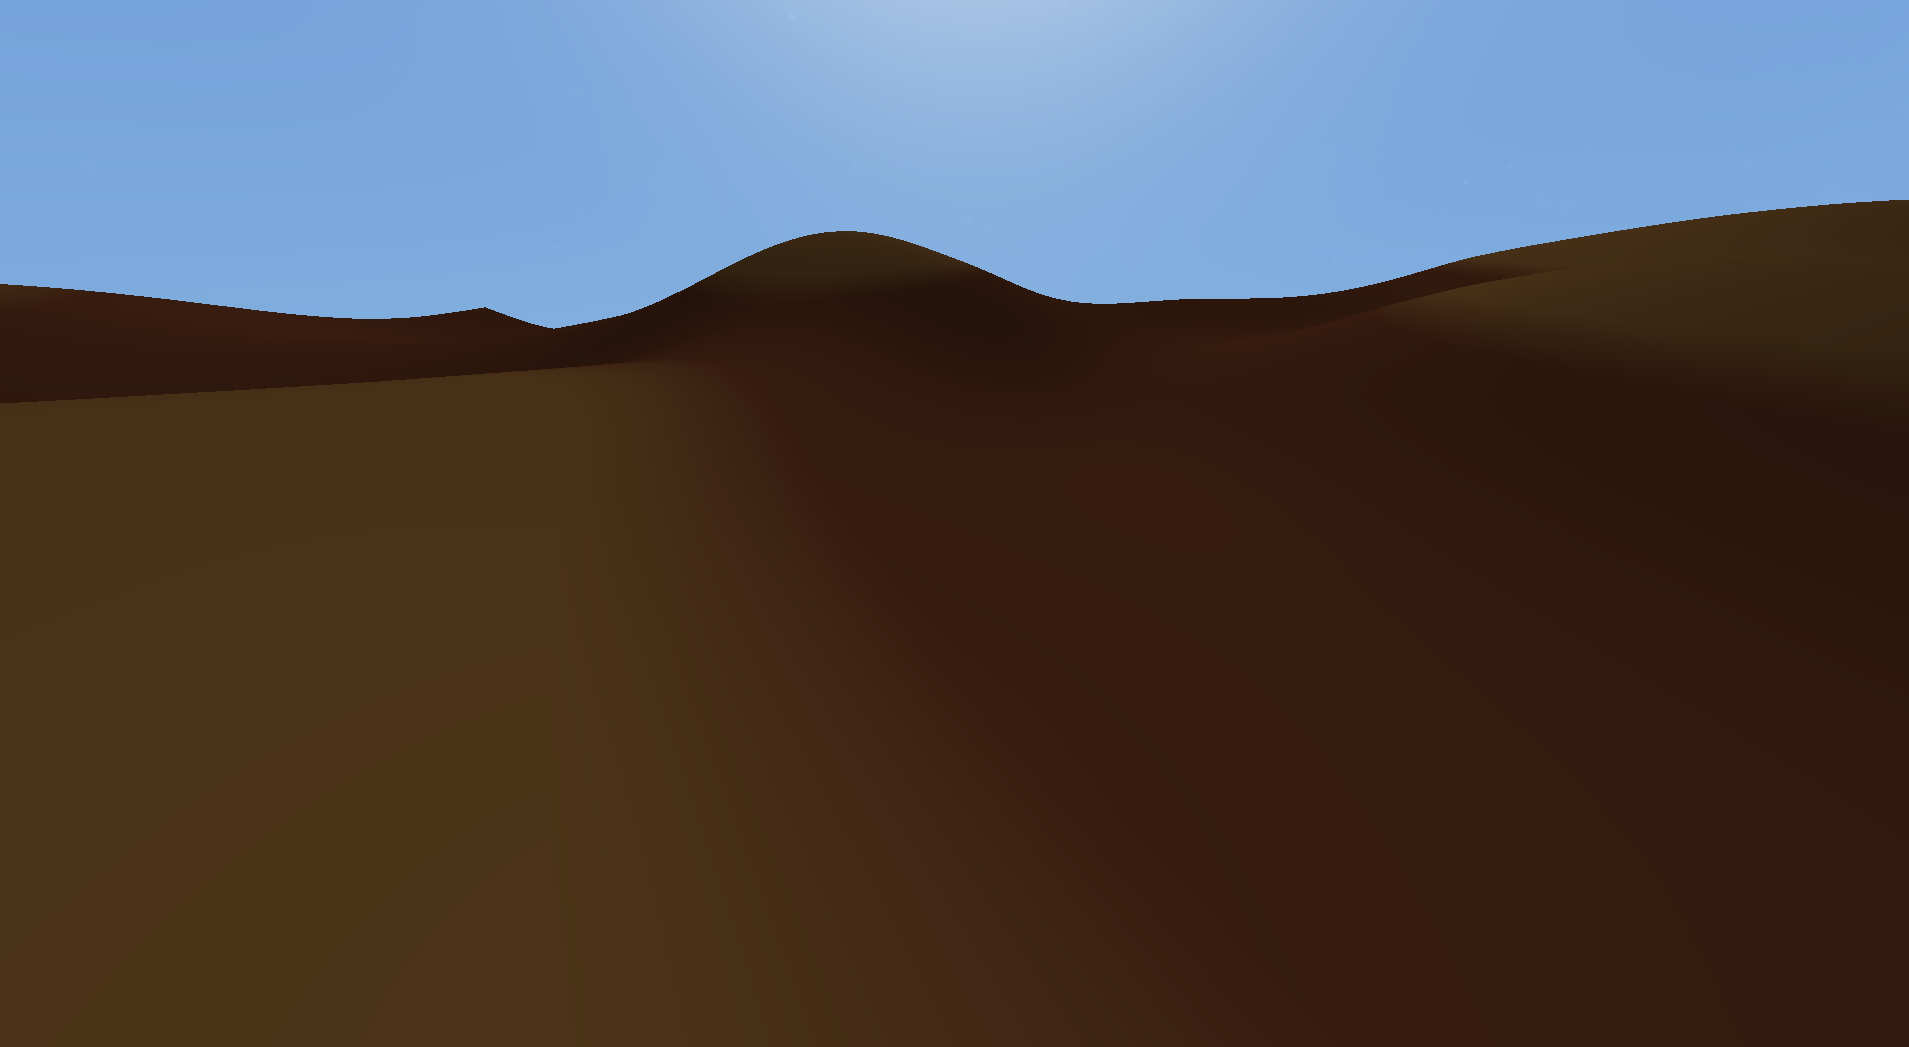
\includegraphics[width=0.8\textwidth]{chapters/system_architecture/sections/terrain/resources/octaves-1.png}
        \caption{Small octaves (1).}
    \end{subfigure}
    \hfill
    \begin{subfigure}{0.45\textwidth}
        \centering
        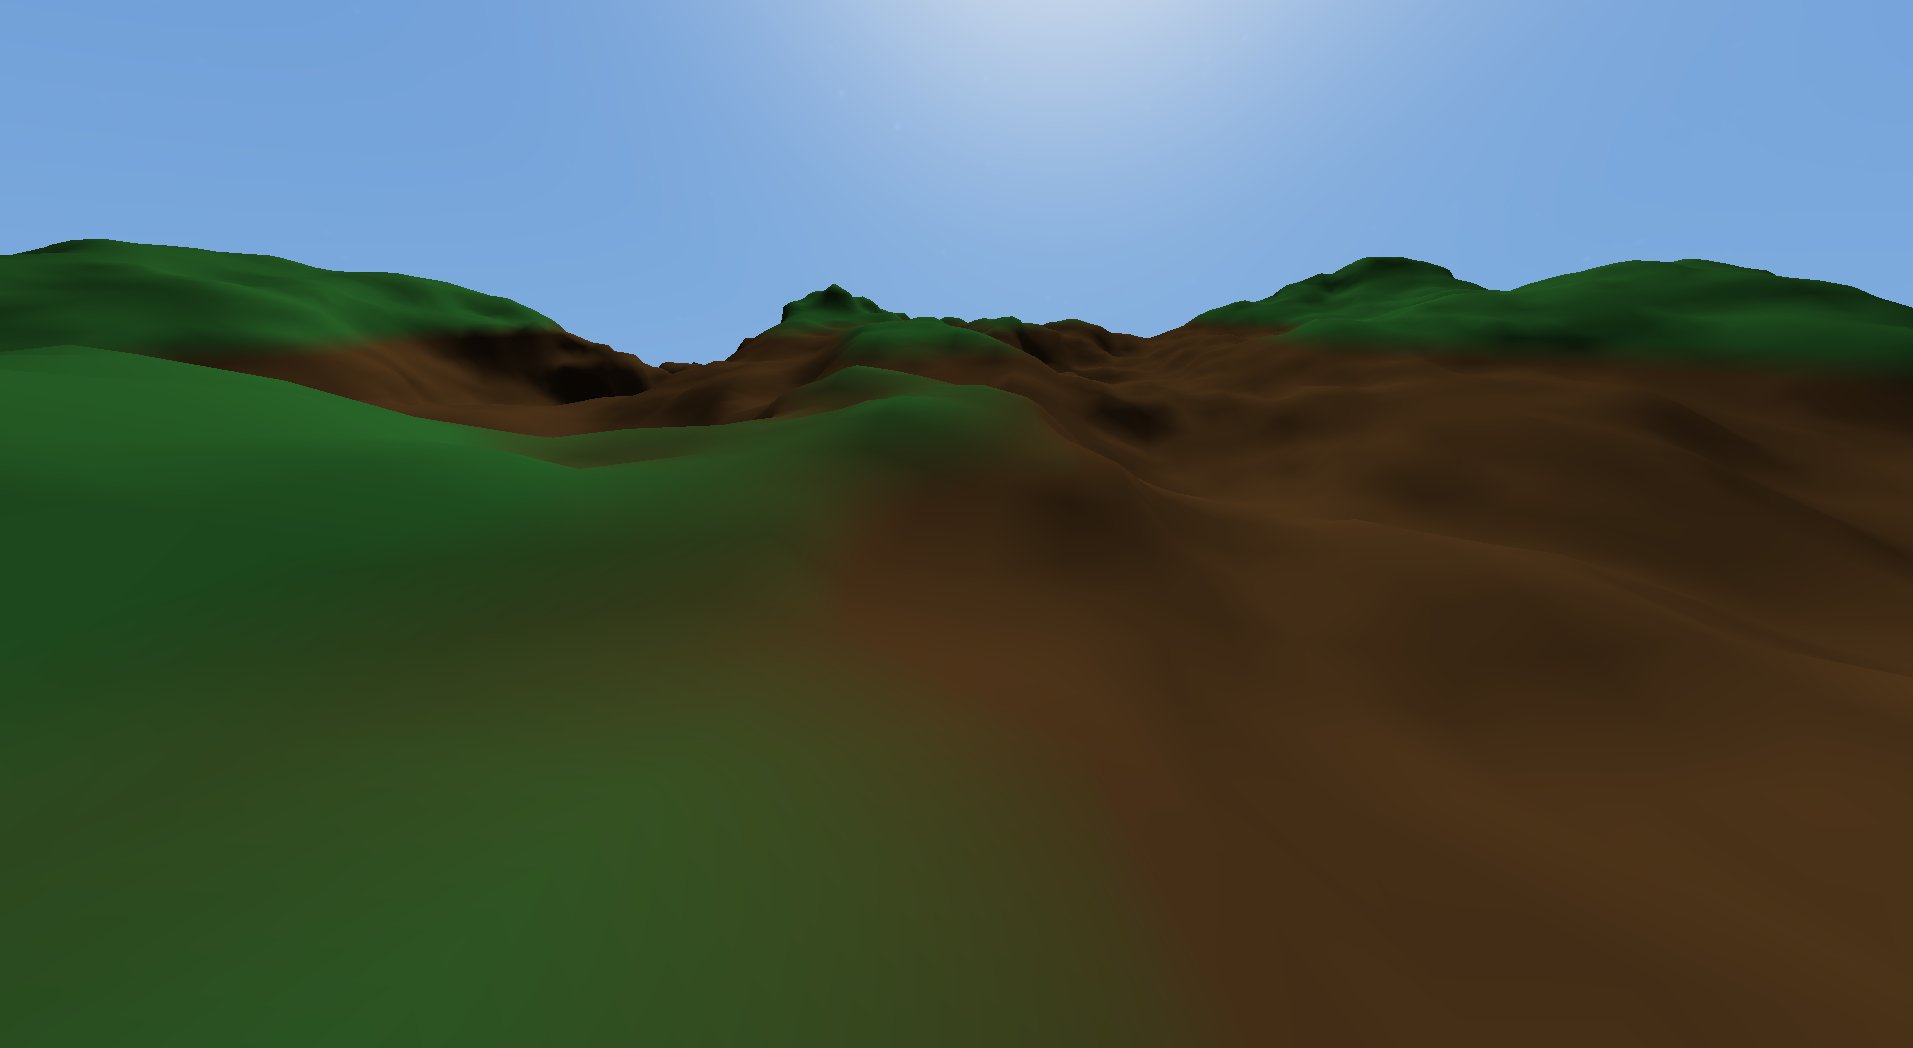
\includegraphics[width=0.8\textwidth]{chapters/system_architecture/sections/terrain/resources/octaves-5.png}
        \caption{Big octaves (5).}
    \end{subfigure}

    \centering
    \begin{subfigure}{0.45\textwidth}
        \centering
        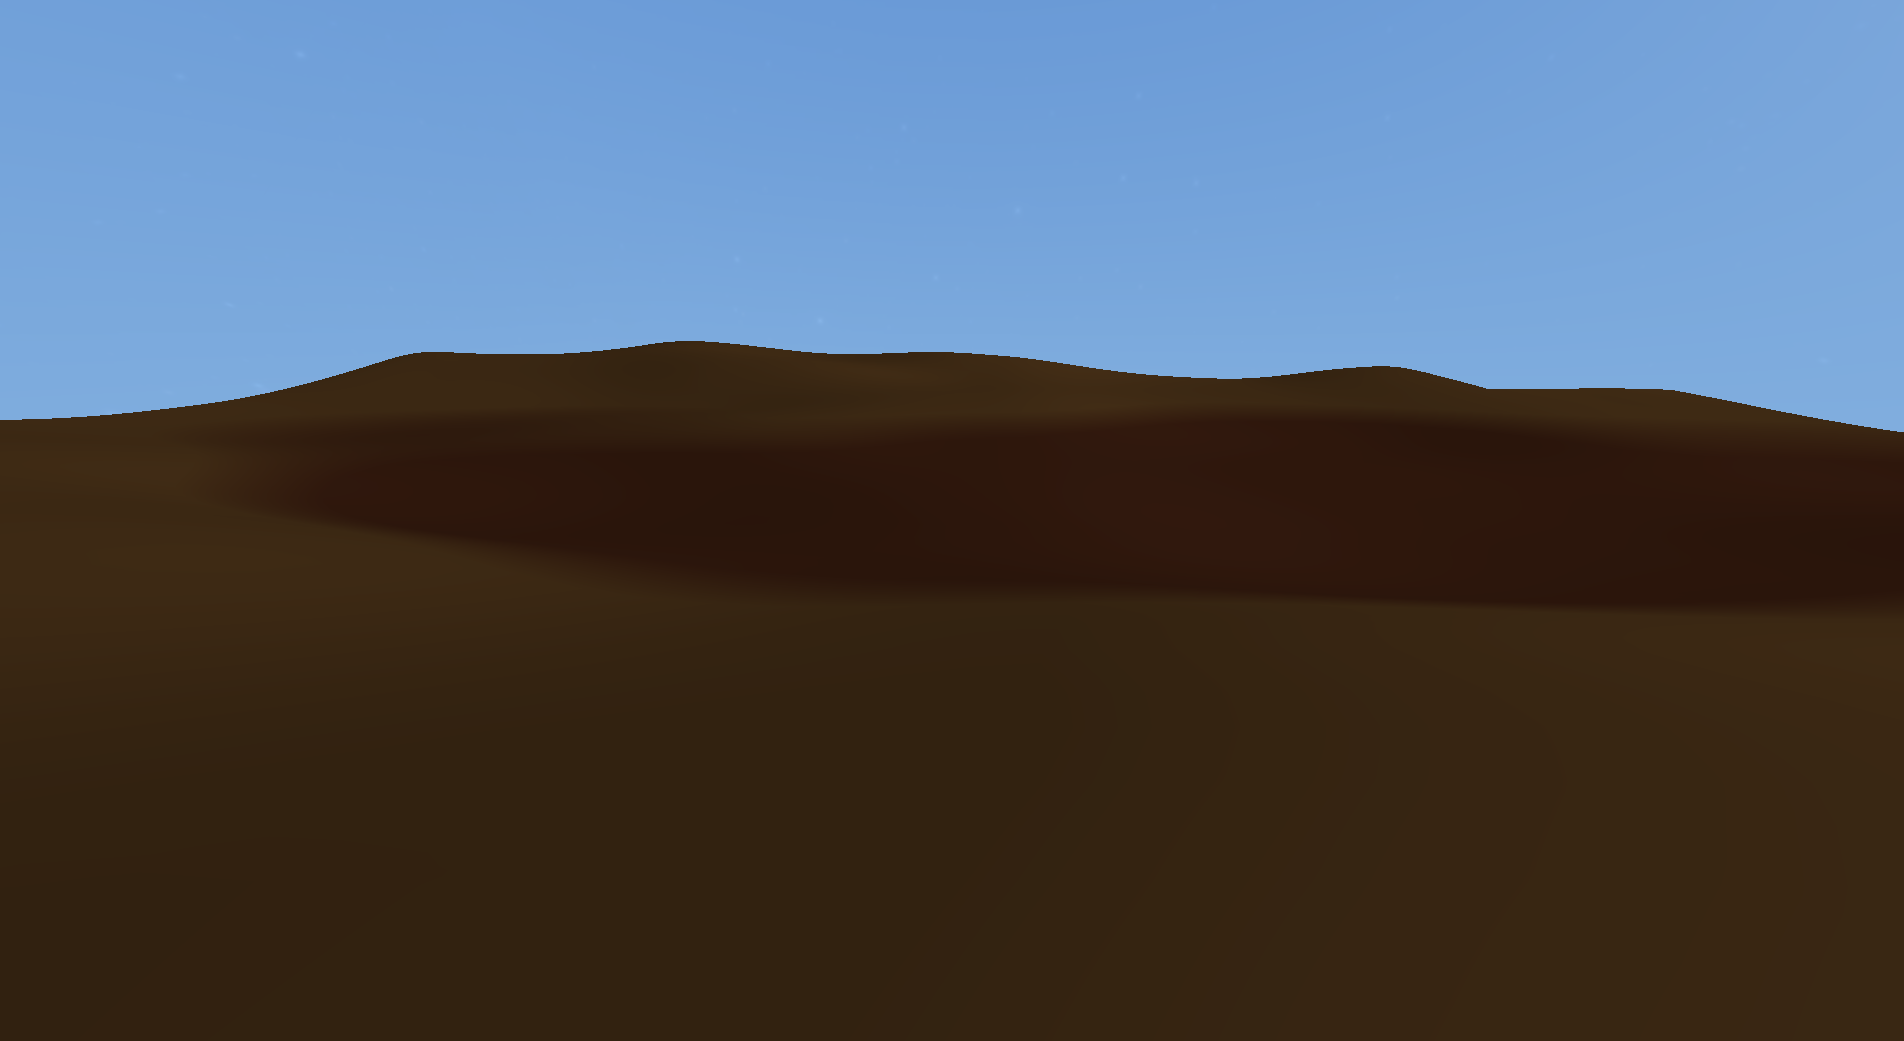
\includegraphics[width=0.8\textwidth]{chapters/system_architecture/sections/terrain/resources/initial-freq-0.1.png}
        \caption{Small initial frequency (1).}
    \end{subfigure}
    \hfill
    \begin{subfigure}{0.45\textwidth}
        \centering
        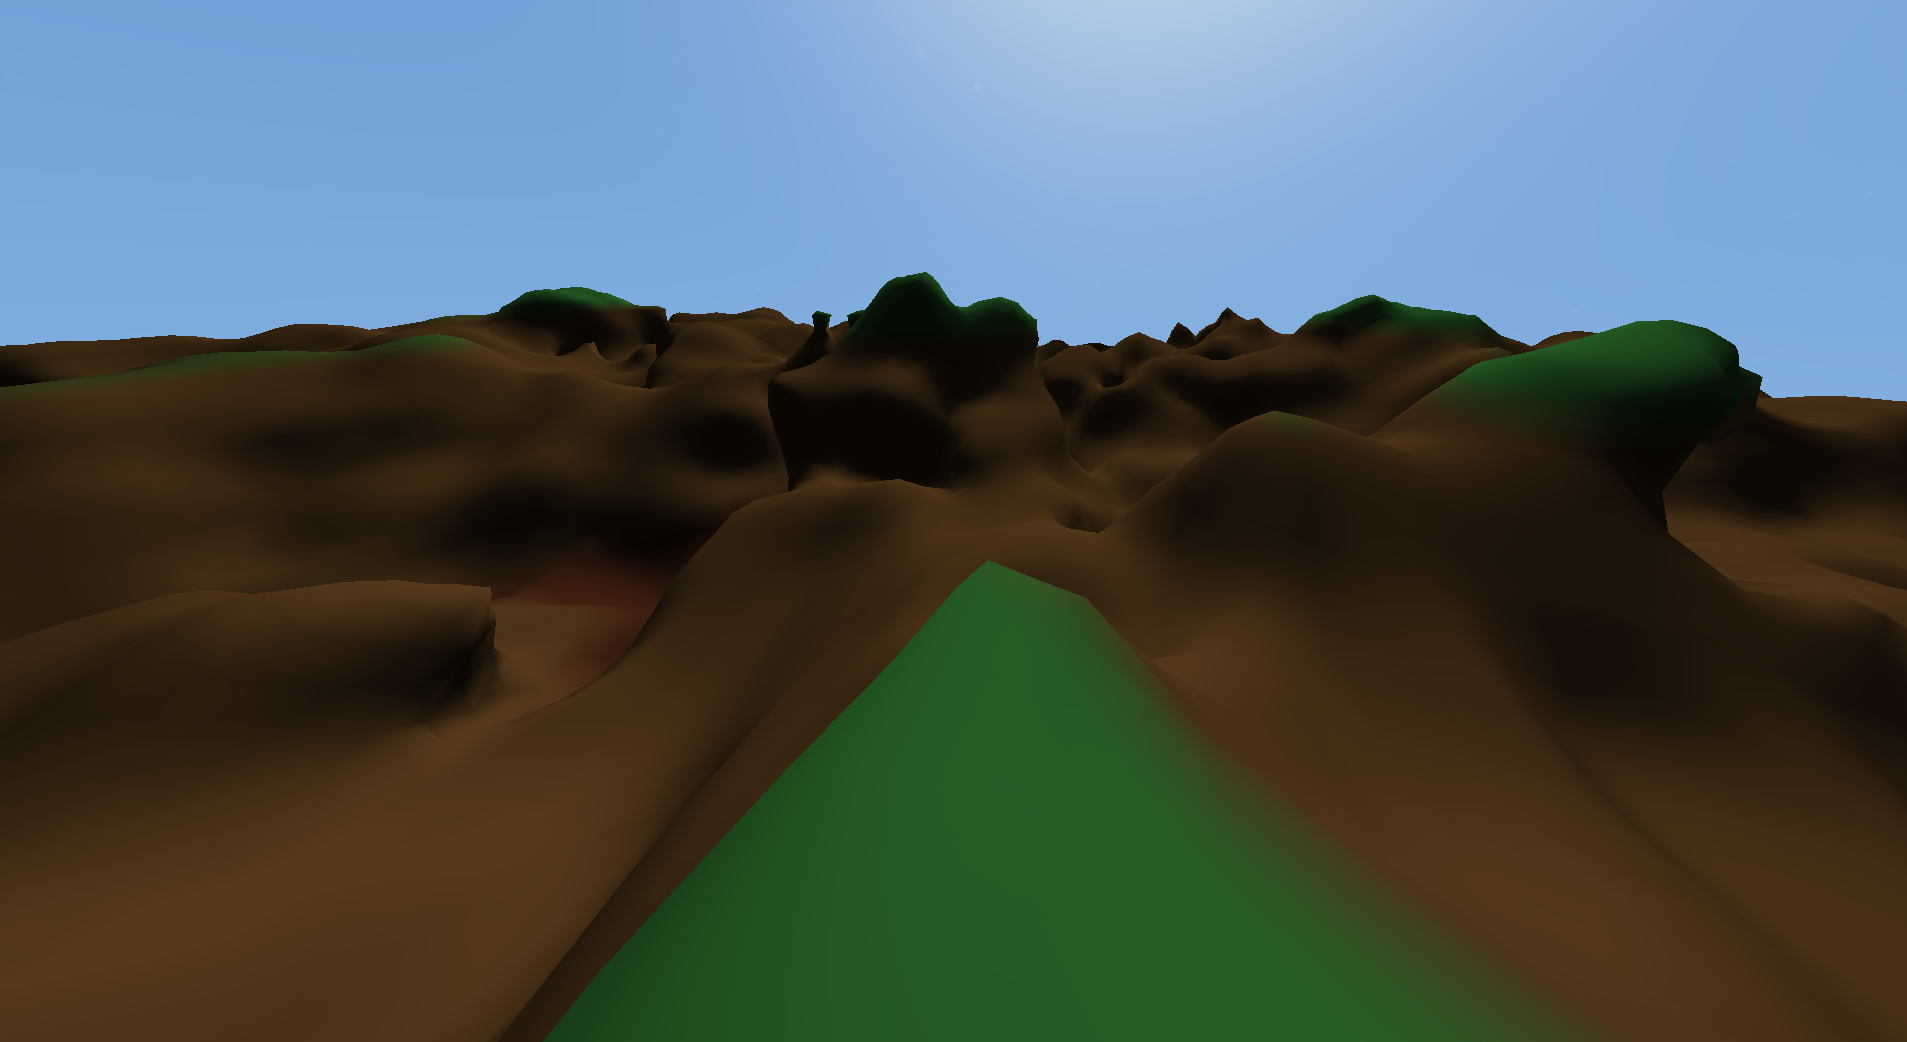
\includegraphics[width=0.8\textwidth]{chapters/system_architecture/sections/terrain/resources/initial-freq-0.5.png}
        \caption{Big initial frequency (0.5).}
    \end{subfigure}

    \centering
    \begin{subfigure}{0.45\textwidth}
        \centering
        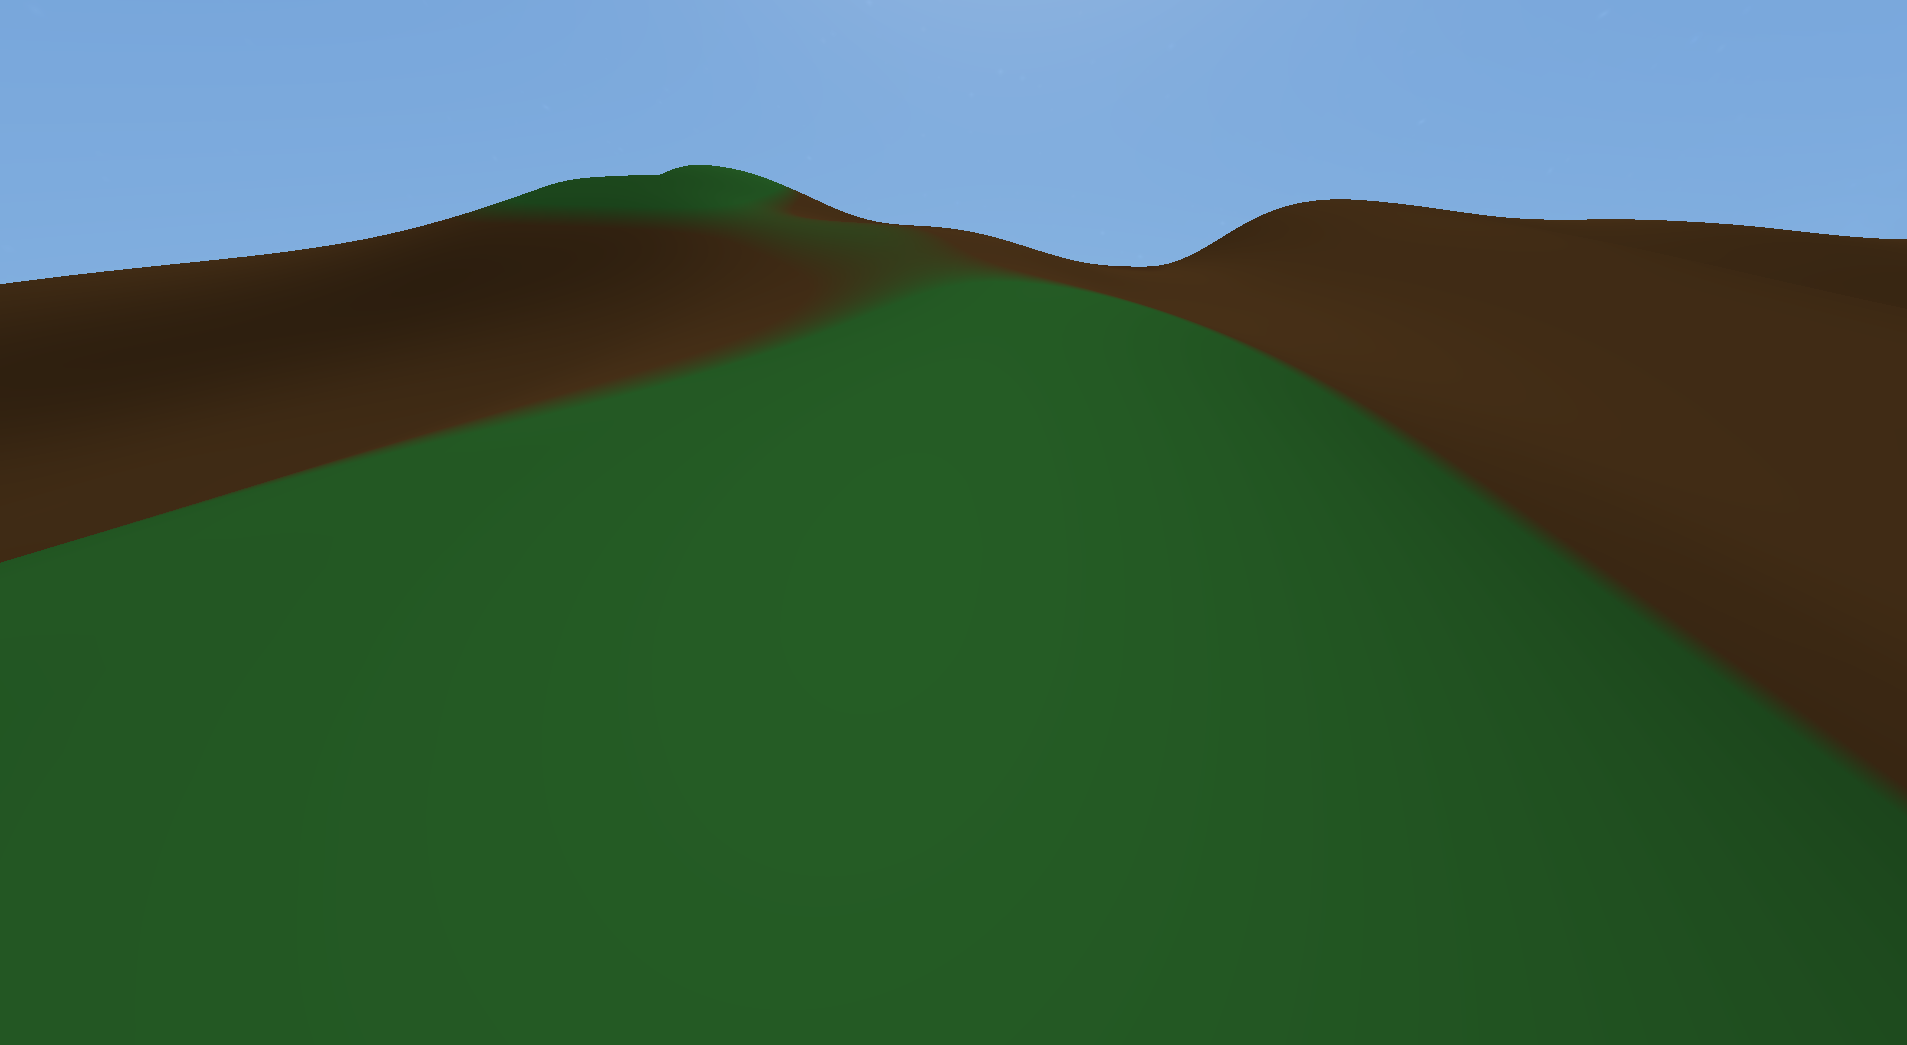
\includegraphics[width=0.8\textwidth]{chapters/system_architecture/sections/terrain/resources/freq-mul-0.5.png}
        \caption{Small frequency multiplier (0.5).}
    \end{subfigure}
    \hfill
    \begin{subfigure}{0.45\textwidth}
        \centering
        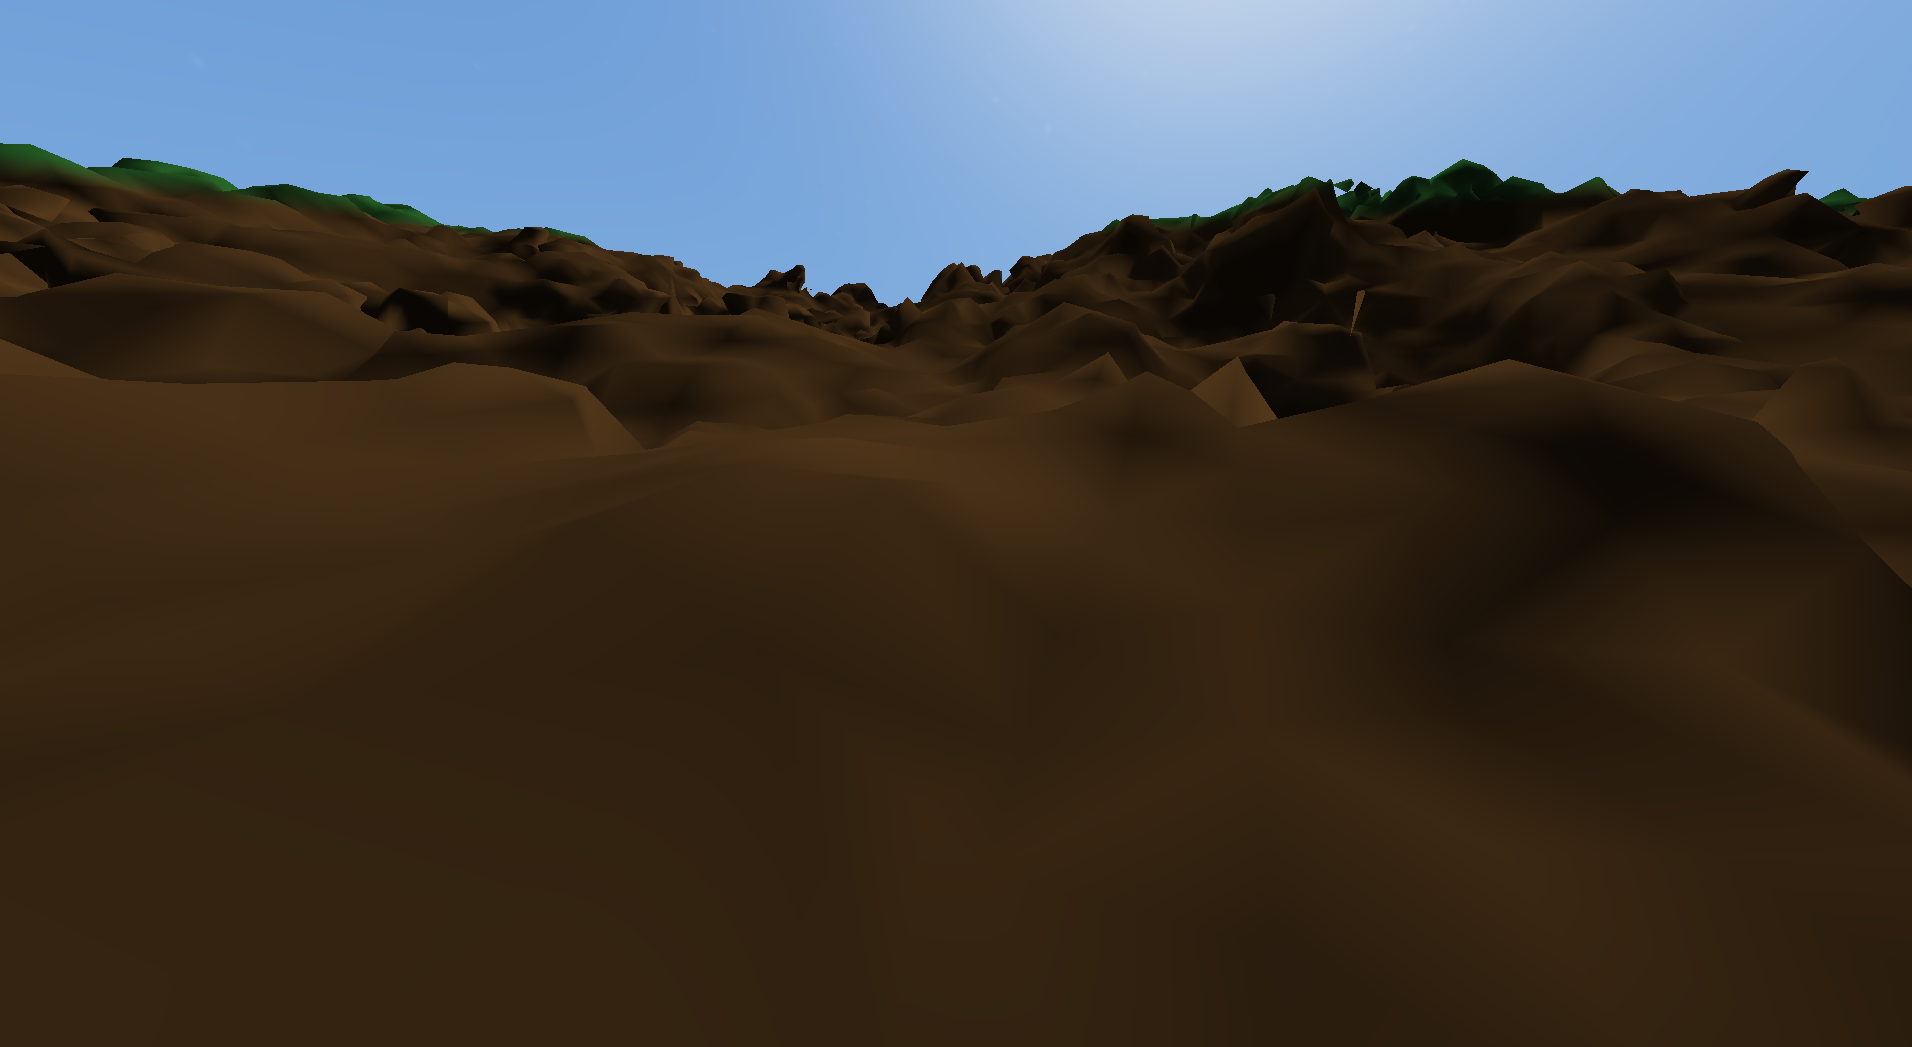
\includegraphics[width=0.8\textwidth]{chapters/system_architecture/sections/terrain/resources/freq-mul-5.png}
        \caption{Big frequency multiplier (5).}
    \end{subfigure}

    \centering
    \begin{subfigure}{0.45\textwidth}
        \centering
        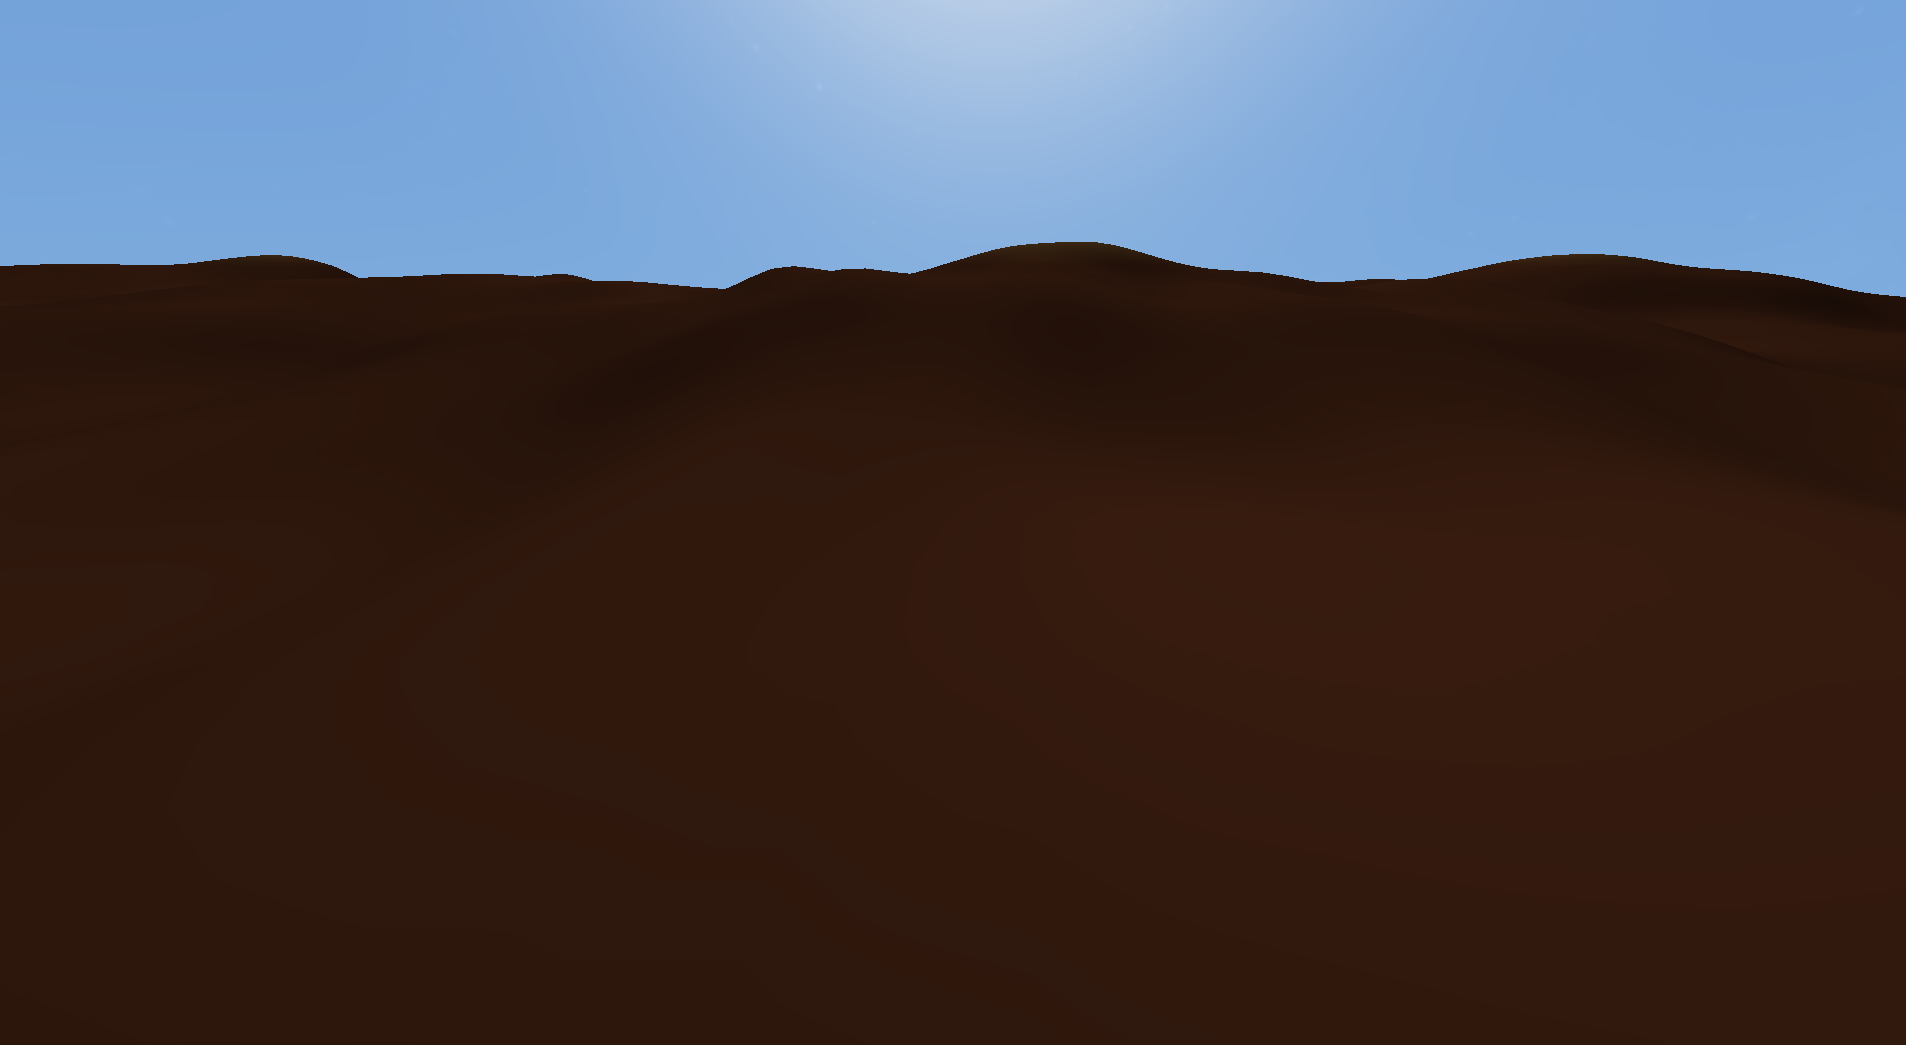
\includegraphics[width=0.8\textwidth]{chapters/system_architecture/sections/terrain/resources/initial-amp-8.png}
        \caption{Small initial amplitude (8).}
    \end{subfigure}
    \hfill
    \begin{subfigure}{0.45\textwidth}
        \centering
        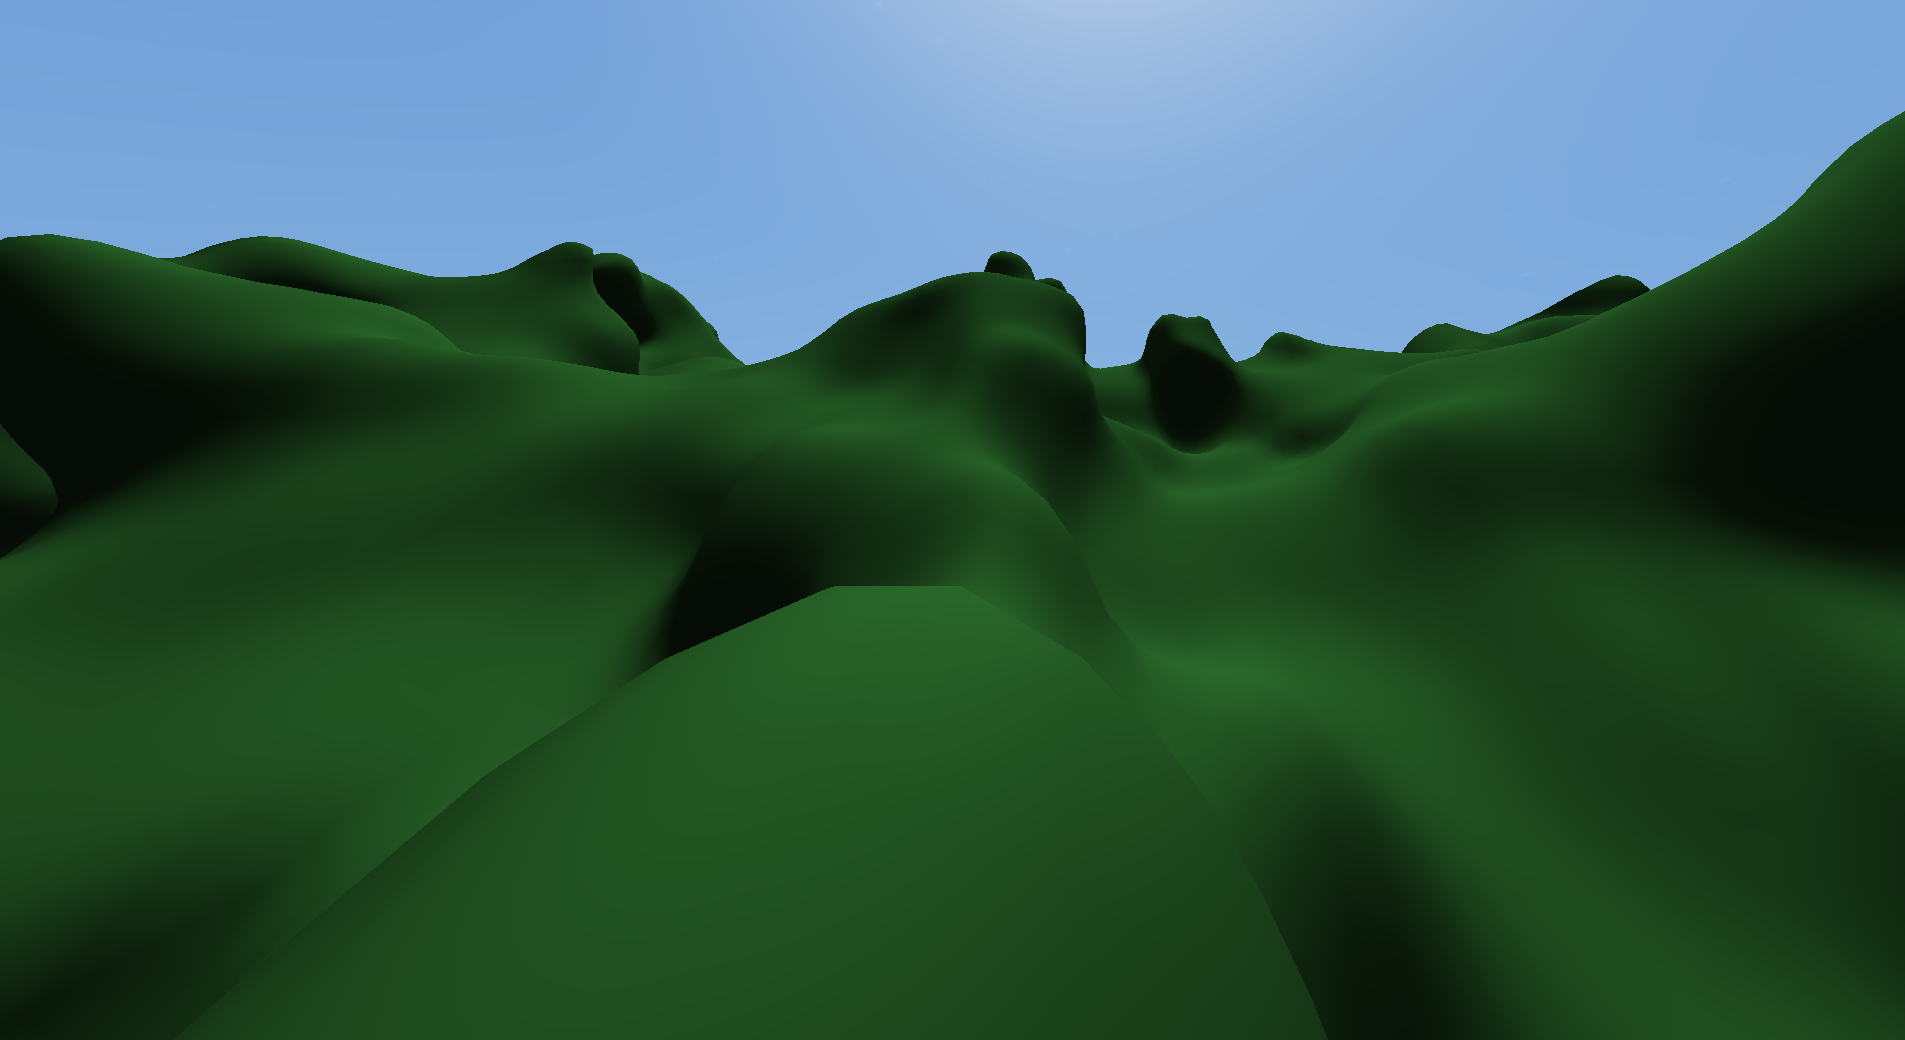
\includegraphics[width=0.8\textwidth]{chapters/system_architecture/sections/terrain/resources/initial-amp-32.png}
        \caption{Big initial amplitude (32).}
    \end{subfigure}

    \centering
    \begin{subfigure}{0.45\textwidth}
        \centering
        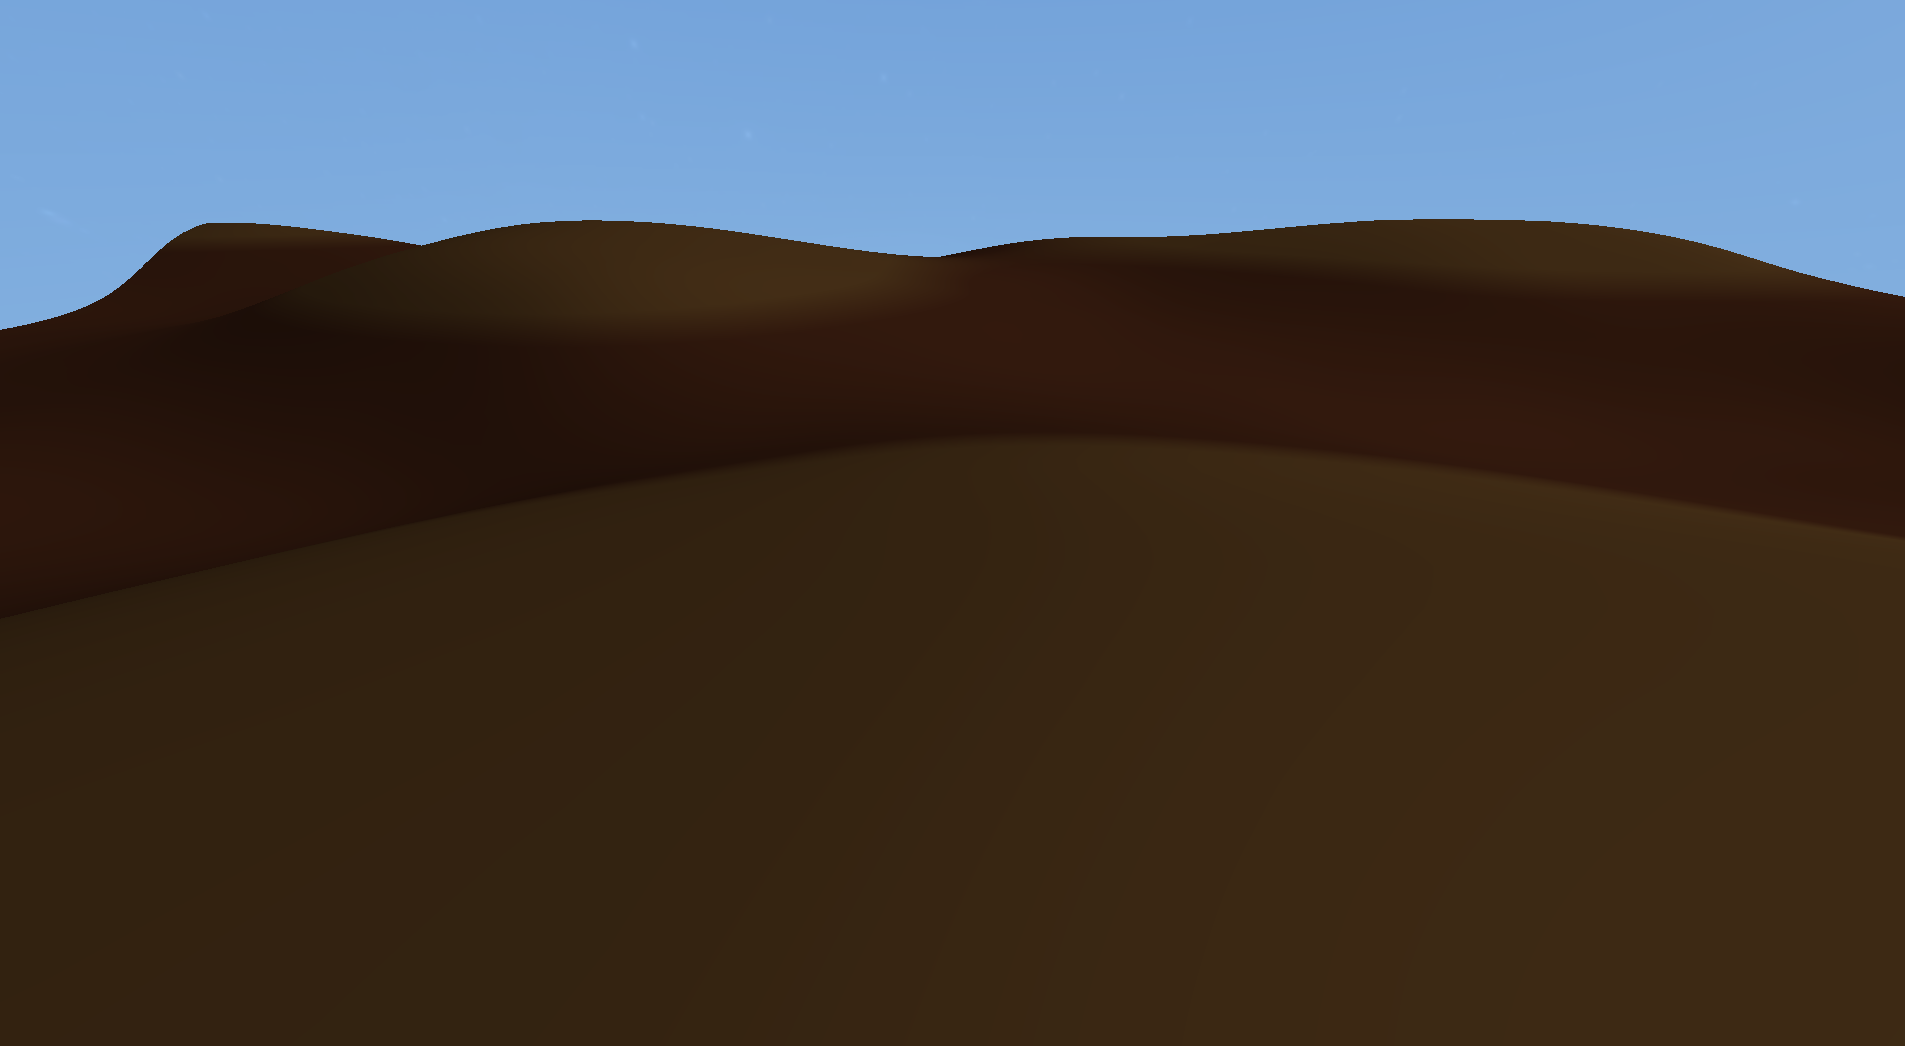
\includegraphics[width=0.8\textwidth]{chapters/system_architecture/sections/terrain/resources/amp-mul-0.1.png}
        \caption{Small amplitude multiplier (0.1).}
    \end{subfigure}
    \hfill
    \begin{subfigure}{0.45\textwidth}
        \centering
        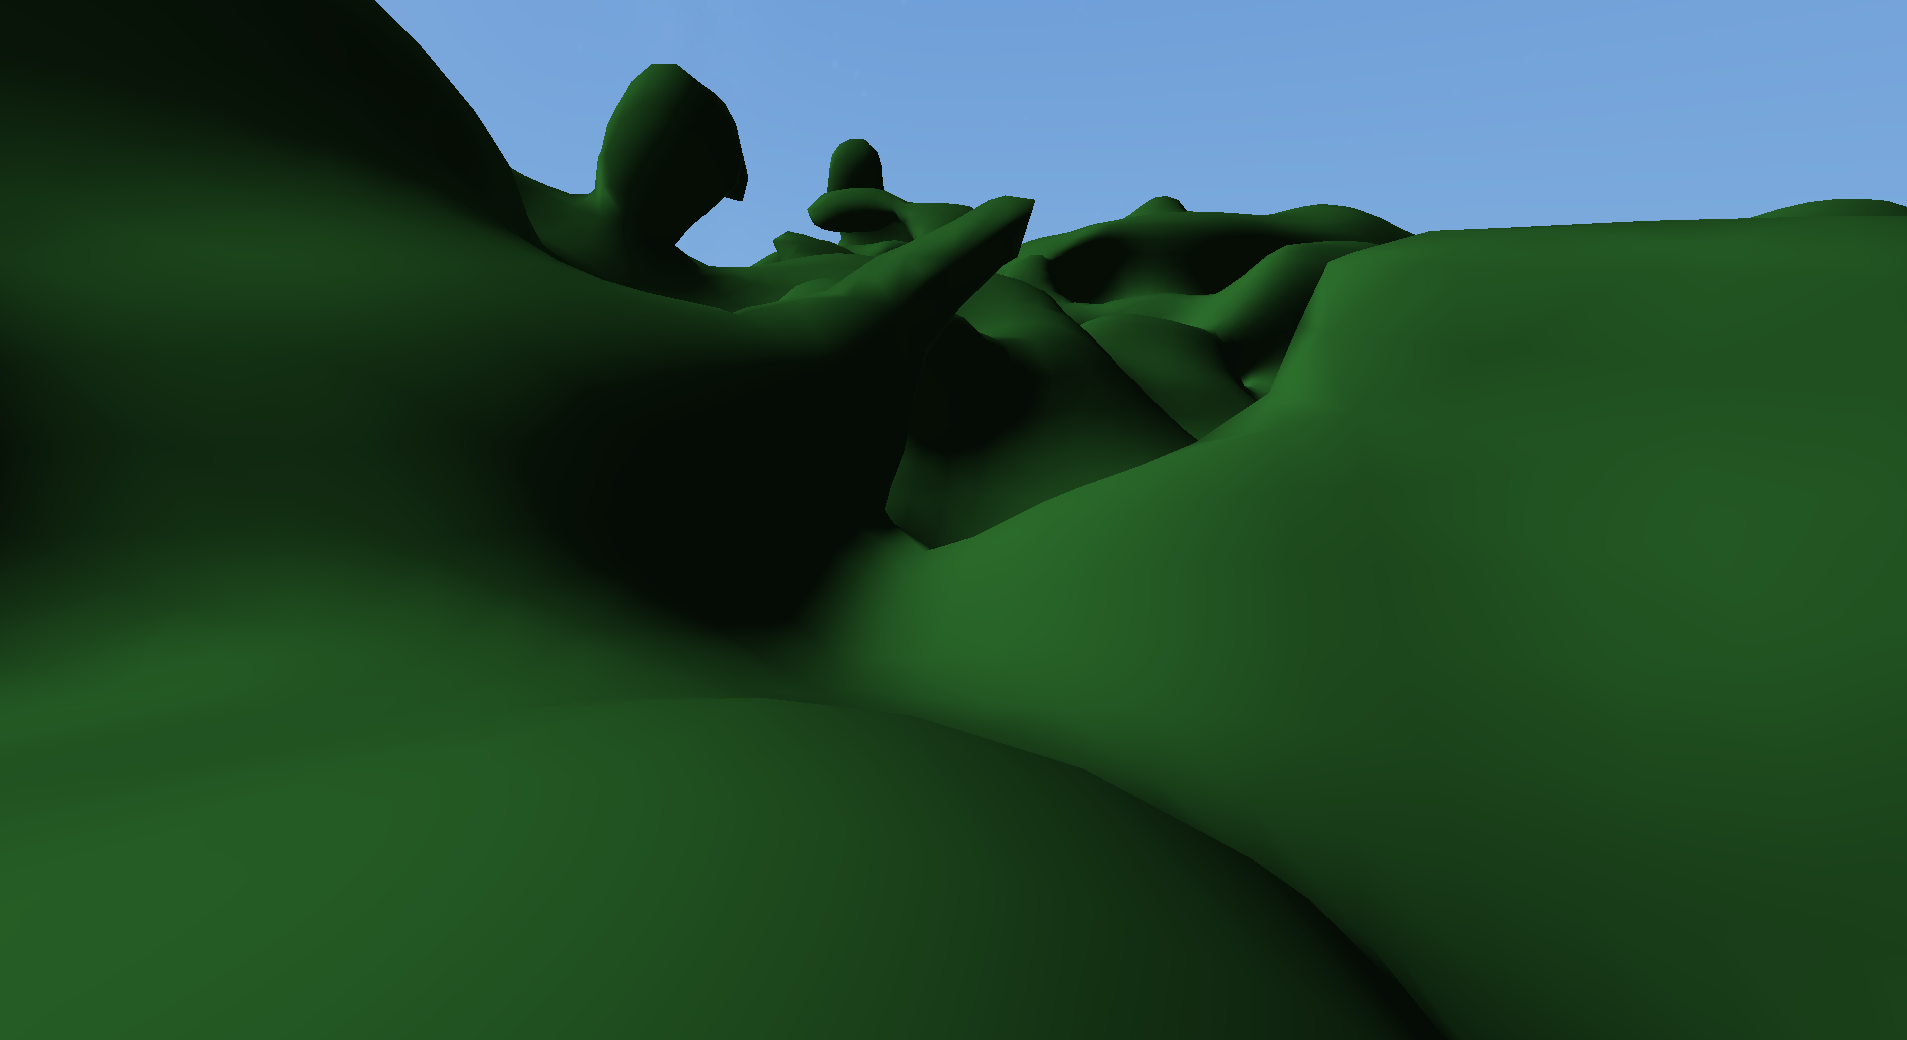
\includegraphics[width=0.8\textwidth]{chapters/system_architecture/sections/terrain/resources/amp-mul-1.png}
        \caption{Big amplitude multiplier (1).}
    \end{subfigure}

    \caption{Scalar field parameter comparison.}
    \label{fig:argument_comparison}
\end{figure}
\subsection{Chunks}
As mentioned before one of the most important things for the terrain was a way to edit it.
Editing the whole terrain at once would be very slow and not very efficient.
Thus the terrain is split into chunks - cubes with side length 16.
Each chunk is a separate object and can be edited independently.
This solution is much more efficient but it also causes some problems.

One problem is that the terrain is not continuous.
Every time we edit a chunk we need to make sure that the edges of the chunk are the same as the edges of the neighboring chunks.
This is done by making sure that when a function that updates one chunk is called it is also called with the same parameters for other affected chunks.
Without this, the terrain would have holes in it between chunks which is shown in a screenshot from an early version of the game in \autoref{fig:gaps_between_chunks}.

Another problem is that the algorithm we used for generating the terrain, described in \autoref{subsec:marching_cubes}, calculates normal vectors based on the values of the scalar field around the point at which the normal is calculated.
This means that the normal vectors at the edges of the chunks have to be calculated differently.
This is a common problem with the algorithm and it is visualized in \autoref{fig:problem_with_normals_at_chunk_edge}.
The most common solution and the one we used is extending the scalar field by one layer of points around the chunk.
This means that the chunk contains information about the scalar field outside of the chunk itself.
That way the normal vectors can be calculated the same way for all points in the chunk.

\begin{figure}[H]
    \centering
    \begin{minipage}{0.45\textwidth}
        \centering
        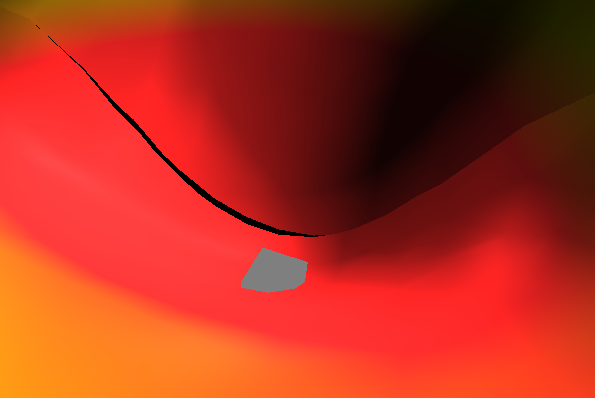
\includegraphics[width=0.8\textwidth]{chapters/system_architecture/sections/terrain/resources/chunk_edges_gaps.png}
        \caption{Gaps between chunks.}
        \label{fig:gaps_between_chunks}
    \end{minipage}\hfill
    \begin{minipage}{0.45\textwidth}
        \centering
        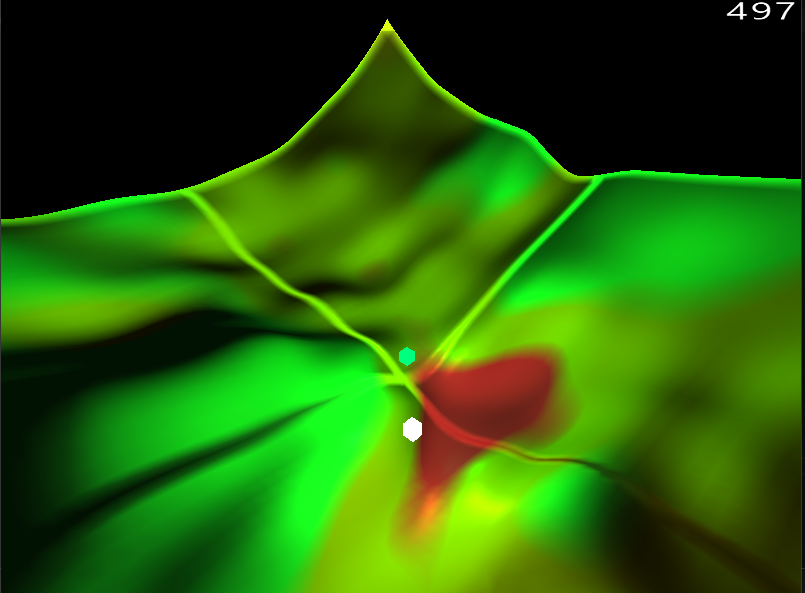
\includegraphics[width=0.8\textwidth]{chapters/system_architecture/sections/terrain/resources/chunk_edges_normals_problem.png}
        \caption{Problem with normals at chunk edges.}
        \label{fig:problem_with_normals_at_chunk_edge}
    \end{minipage}
\end{figure}

There are infinitely many chunks in the world, which is why chunks are only loaded when a player is close to them.
They are also unloaded when the player moves far enough away from them.
When that happens they are saved to disk and removed from RAM.
The same thing happens when the game is closed.
\subsection{Marching Cubes} \label{subsec:marching_cubes}
The idea of the algorithm is described in \autoref{sec:theory_theory_marching_cubes}.
This section will describe the way the algorithm was implemented in our project.

To make the mesh look smoother we interpolate the position of the vertices on the edges based on the values of the scalar field at the vertices.
This is done by using the linear interpolation given by equation \autoref{eq:linear_interpolation}.
\begin{equation}
  \label{eq:linear_interpolation}
  P = V_1 + \frac{\text{IsoLevel} - v_1}{v_2 - v_1} \times (V_2 - V_1)
\end{equation}
where $P$ is the resulting position of the vertex, $V_1$ and $V_2$ are the positions of the vertices on the edge, $v_1$ and $v_2$ are the values of the scalar field at the vertices and IsoLevel is the isolevel of the mesh.
  
This gives us a mesh.
To make the impression of a light reflecting off a smooth surface we also need to calculate the normal vectors for each vertex.
The normal vectors for each vertex of the scalar field are calculated using \autoref{eq:normal_vector}
\begin{equation}
    \label{eq:normal_vector}
    n(x, y, z) = \begin{bmatrix}
        s(x + 1, y, z) - s(x - 1, y, z) \\
        s(x, y + 1, z) - s(x, y - 1, z) \\
        s(x, y, z + 1) - s(x, y, z - 1)
      \end{bmatrix}
\end{equation}
where $s(x, y, z)$ is the scalar field function and $n$ is the normal vector.
These vectors are used to calculate the mesh normals using the same interpolation used for the mesh \autoref{eq:linear_interpolation}.

The last part of creating the mesh is assigning the colors to each vertex.
Each vertex of the scalar field is assigned a type which is described in \autoref{subsec:scalar_field}.
Each type has a color assigned to it.
The color of each vertex of the mesh is calculated by interpolating the colors of the vertices of the scalar field using \autoref{eq:linear_interpolation}.


\subsection{Editing terrain} \label{sec:terrain_editing}
Editing terrain is done by changing the values of the scalar field.
When a chunk is first created the values of the scalar field are calculated for each point in the chunk and then saved.
This allows for the scalar field values to be edited.
When a chunk is edited the values of the scalar field are recalculated for the edited points and the points around them.
The player can choose a point to build or mine at.
Values of the scalar field close to that point are then changed based on the pickaxe the player uses and how long they mine for.
The closer the point to the chosen point the more it is affected.
A 3D Gaussian function is used to calculate exactly how much each point is affected.
The function is shown in \autoref{eq:gaussian}.

\begin{equation}
    \label{eq:gaussian}
    f(x,y,z) = e^{-a \left((p_x - c_x)^2 + (p_y - c_y)^2 + (p_z - c_z)^2\right)}
\end{equation}

In \autoref{eq:gaussian} $p_x$, $p_y$ and $p_z$ are the coordinates of the point being edited, $c_x$, $c_y$ and $c_z$ are the coordinates of the chosen point and $a$ is a constant.
Moreover, if the distance between the chosen point and the point being edited is greater than the range of the pickaxe, the point is not affected.

Once the values of the scalar field are updated the chunk is regenerated.
This is a very time-consuming process which is why it was moved to a second thread.
The communication between that thread and the main one is described in: \todo{Describe chunk worker}
